\chapter{Esquema eléctrico}\label{cap:esquema}

\begin{figure}[H]\centering
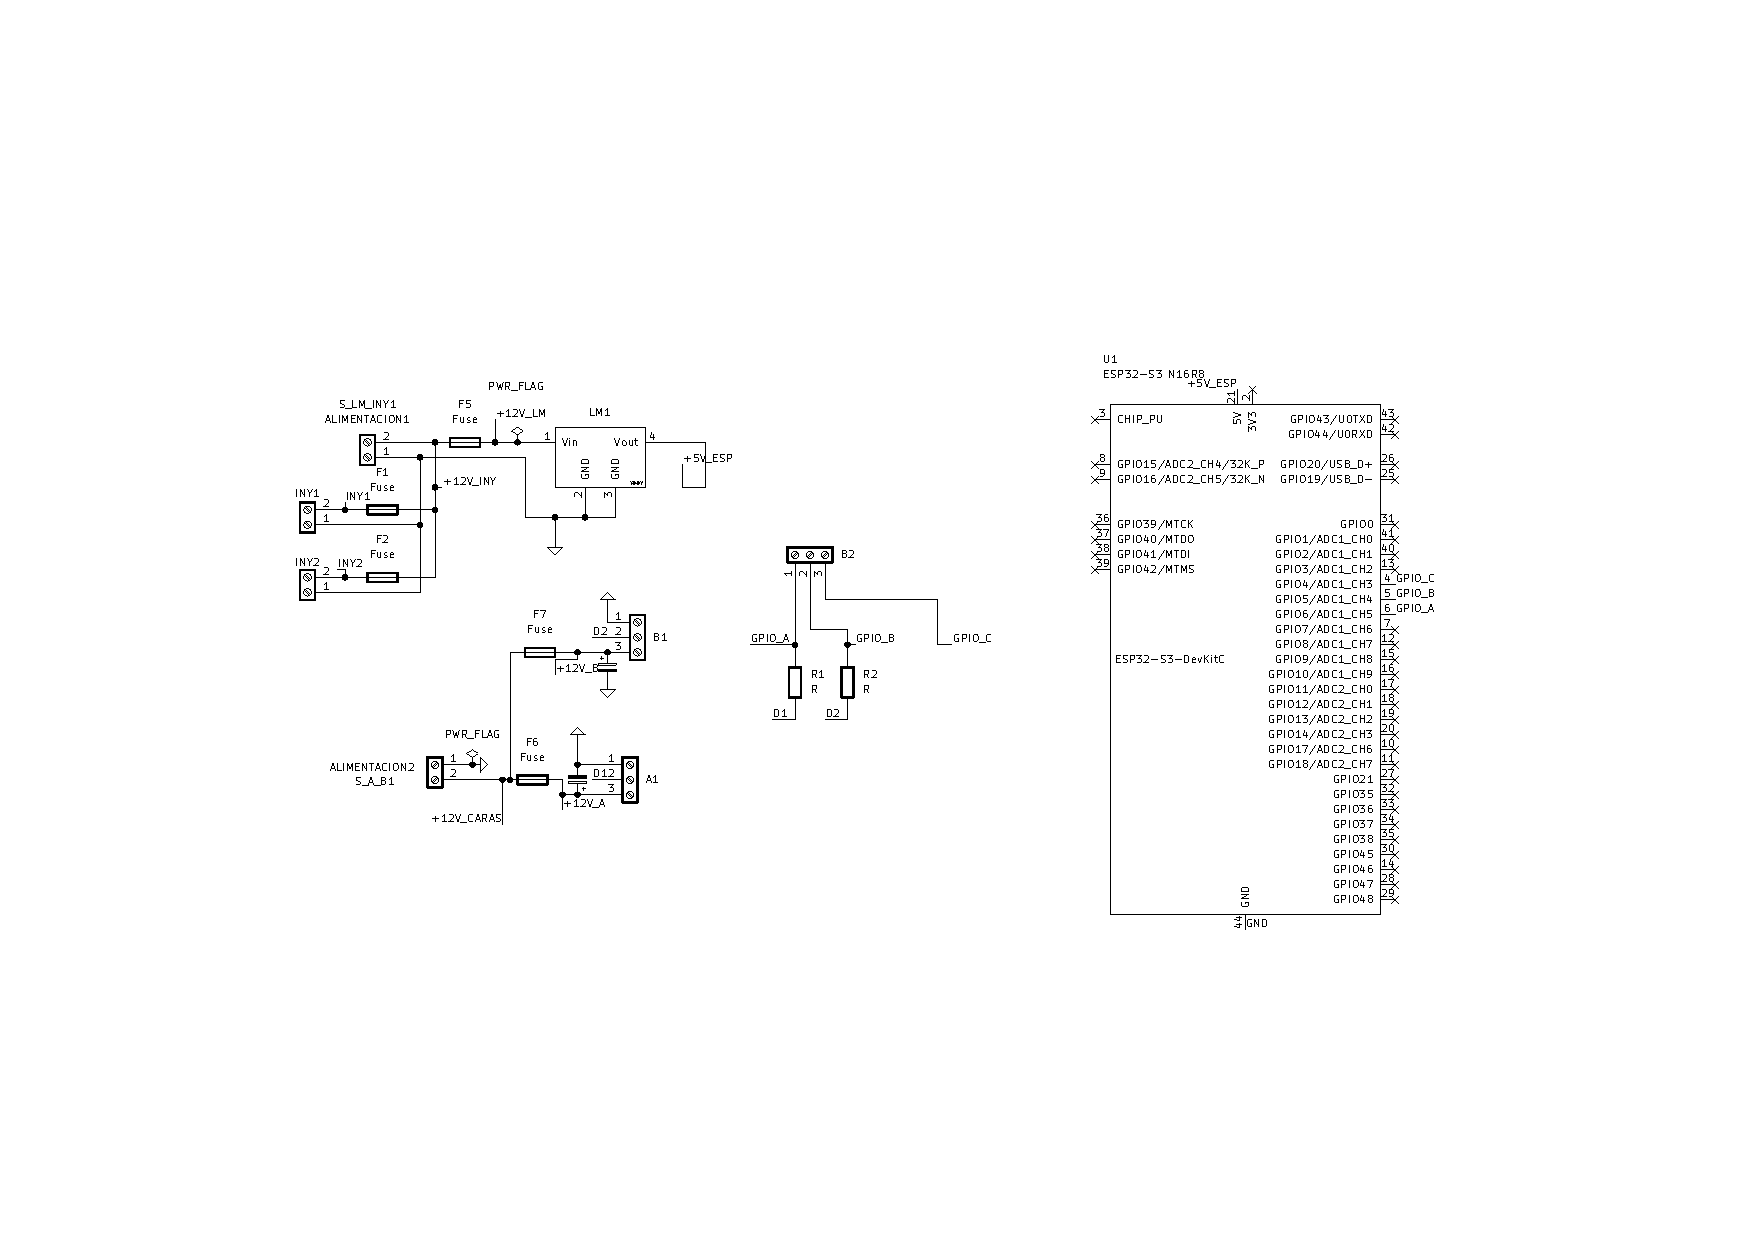
\includegraphics[width=\linewidth, trim=133 141 145 162, clip]{img/pcb/esquema.pdf}
\caption{Esquema de la \dato{pcbVersion}, exportado de KiCad. El PDF original (\texttt{PCB\_V2\_schematic.pdf}) va en los entregables para ampliarlo.}\label{fig:esquema}
\end{figure}

\section{Bloques del esquema}

\begin{description}[leftmargin=0pt]
\item[Alimentación del regulador e inyección] S\_LM\_INY1 entrega +12~V a la red \texttt{+12V\_INY}, que pasa por F5 (puenteado) hacia la entrada del LM2596 y hacia F1 (INY1) y F2 (INY2).
\item[Regulador] El LM2596 entrega \dato{reguladorSalida} en \texttt{+5V\_ESP}, conectado al pin 5V de la ESP32.
\item[Alimentación de las caras] S\_A\_B1 entrega +12~V a \texttt{+12V\_CARAS}; F6 alimenta la cara A (A1) y F7 la cara B (B1). C1 y C2 filtran cada salida.
\item[Datos] Tres pines de la ESP32 llegan a la bornera B2 como \texttt{GPIO\_A}, \texttt{GPIO\_B} y \texttt{GPIO\_C}. \texttt{GPIO\_A} pasa por R1 a \texttt{D1} (cara A) y \texttt{GPIO\_B} por R2 a \texttt{D2} (cara B). \texttt{GPIO\_C} queda libre para una función futura.
\end{description}

\section{Pines de datos}\label{sec:pines}

En el proyecto existen tres versiones de qué pin de la ESP32 lleva los datos de cada cara:

\begin{tabularx}{\linewidth}{@{}l X X X@{}}
\toprule
\textbf{Señal} & \textbf{Esquema de KiCad (PCB\_V2)} & \textbf{Nota del proyecto (LEEME)} & \textbf{Poste funcionando hoy} \\ \midrule
Datos cara A & \texttt{GPIO\_A} → pin 6 del módulo (GPIO\dato{pinesEsquema.GPIO_A}) & GPIO4 & GPIO\dato{pinesPosteActual.caraA}, \dato{driverCaraA} \\
Datos cara B & \texttt{GPIO\_B} → pin 5 del módulo (GPIO\dato{pinesEsquema.GPIO_B}) & GPIO5 & GPIO\dato{pinesPosteActual.caraB}, \dato{driverCaraB} \\
Reserva & \texttt{GPIO\_C} → pin 4 del módulo (GPIO\dato{pinesEsquema.GPIO_C}) & GPIO7 & --- \\
\bottomrule
\end{tabularx}

\pendiente{pinesConfirmados}{Qué GPIO lleva realmente los datos de cada cara en la placa fabricada. El esquema, la nota del proyecto y el poste que funciona no coinciden. En el poste que funciona se comprobó además que el camino de la placa hacia GPIO18 no da señal y que la cara B solo funciona en GPIO3 con el driver I2S. Hasta confirmarlo, configura WLED con los pines del poste que funciona (\dato{pinesPosteActual.caraA} y \dato{pinesPosteActual.caraB}) y comprueba la placa con el procedimiento de la sección~\ref{sec:comprobar-pin}.}

\section{Cómo comprobar el pin en una placa}\label{sec:comprobar-pin}

Con la placa \textbf{sin alimentación}:
\begin{enumerate}
\item Pon el multímetro en continuidad.
\item Una punta en el borne 2 (datos) de A1. La otra, en el lado de R1 que no va a A1. Debe sonar: ese es el lado \texttt{GPIO\_A}.
\item Deja una punta en ese lado de R1 y recorre con la otra los pines del módulo ESP32 hasta que suene.
\item Lee el nombre del pin en la serigrafía del propio módulo ESP32 (no en la de la PCB). Ese es el GPIO de la cara A.
\item Repite con B1, R2 y la cara B.
\item Si la cara B no enciende con su GPIO en WLED, cambia esa salida al driver I2S (capítulo~\ref{cap:wled}).
\end{enumerate}

\nota{La serigrafía del módulo manda: algunas placas ESP32-S3 compatibles ordenan los pines distinto a la DevKitC oficial de Espressif, que es la que usa la huella de KiCad.}
